%! Author = Yilin
%! Date = 2025/1/27

The distribution of cybercrime is closely tied to national demographic statistics,
with the number of cybercrime incidents showing a positive correlation with several key factors.
In this section, we explore the relationship between cybercrime and four primary demographic indicators:
the proportion of internet users in a country,
the country's GDP, and the proportion of the population with higher education.
By analyzing these factors,
we aim to uncover patterns and correlations that can provide insights into the drivers of cybercrime
and inform the development of more targeted and effective cybersecurity policies.
\subsection{Data Preprocessing}\label{subsec:data-preprocessing} %5.1
    To analyze the correlation between national demographics and cybercrime distribution,
    we first preprocess the relevant data.
    The demographic indicators—internet user penetration\cite{it-net-user-zs}, 
    GDP\cite{ny-gdp-mktp-cd} and 
    the proportion of the population with higher education\cite{se-ter-enrr}
    —are obtained from the World Bank's official website.
    Additionally, we utilize the annual cybercrime incident data for each country,
    which was previously processed in our earlier analysis.
    By integrating these datasets,
    we ensure a comprehensive foundation for examining the relationship between demographic factors and cybercrime trends.
    \begin{itemize}[label=\phantom{.}, leftmargin=-0.18em]
        \item \textbf{Data Integration and Cleaning}: \\
            For each dataset, we filter the data to include only the years from 2010 to 2022.
            After filtering,
            we handle missing values by allowing a maximum missing value proportion of 20\% for each country's data.
            Missing values within this threshold are filled using linear interpolation.
            Any data points that remain missing after interpolation
            are removed to ensure the integrity and reliability of the dataset.
            This preprocessing step ensures that our analysis is based on a consistent and high-quality dataset.
    \end{itemize}


\subsection{Data Processing and Analysis}\label{subsec:data-processing-and-analysis} %5.2
    \subsubsection{Data Consolidation} %5.2.1
        After preprocessing the individual datasets, we integrate the internet user data and the cybercrime incident data.
        This is achieved by performing an inner join on the two datasets using country codes and years as the matching keys.
        The inner join ensures that only the countries and years present in both datasets are retained,
        resulting in a combined dataset where each entry corresponds to a specific country and year with complete data
        for both internet user penetration and cybercrime incidents.
        This step is crucial for ensuring the accuracy and consistency of our subsequent analysis.

    \subsubsection{Logarithmic Transformation} %5.2.2
        To address the skewness in the distribution of cybercrime incident counts,
        we apply a logarithmic transformation to the data.
        As described in Subsection~\ref{subsec:building-the-hotspot-map},
        we use the \textit{log1p} transformation, which computes the natural logarithm of \(1 + x\),
        where \(x\) is the original cybercrime count.
        This transformation reduces the impact of extreme values and makes the data more symmetric,
        bringing it closer to a normal distribution.
        By applying this transformation, we ensure that the data is better suited for statistical analysis and modeling.

    \subsubsection{Spearman Correlation Analysis} %5.2.3
        To quantify the relationship between those data and the number of cybercrime incidents,
        we calculate the Spearman correlation coefficient.
        This non-parametric measure assesses the strength and direction of the monotonic relationship between two variables.
        The Spearman correlation coefficient (\(\rho\)) and its associated \(p\)-value are computed,
        with the \(p\)-value used to determine the statistical significance of the correlation.
        A \(p\)-value smaller than \(1 \times 10^{-10}\) indicates an extremely strong statistical significance.
        The Spearman correlation coefficient is calculated as follows:
        \[ \rho = 1 - \frac{6 \sum d_i^2}{n(n^2 - 1)} \]
        where:
        \begin{itemize}
            \item \(\rho\) is the Spearman rank correlation coefficient,
            \item \(d_i\) is the difference between the ranks of each pair of observations, and
            \item \(n\) is the number of observations.
        \end{itemize}

\subsection{Data Visualization}\label{subsec:data-visualization} %5.3
To further explore the relationship between demographic factors and cybercrime,
we generate several visualizations.
These include scatter plots, time series plots, and distribution plots,
all of which are presented on a logarithmic scale
due to the logarithmic transformation applied during data preprocessing.

    \subsubsection{Scatter Plots} %5.3.1
        We begin by plotting scatter diagrams to visualize the relationship between demographic indicators
        (such as internet user penetration, higher education enrollment, and GDP) and the logarithmically transformed cybercrime counts.
        A regression line is added to each scatter plot to highlight the trend.
        The Spearman correlation coefficient (\(\rho\)) and its associated \(p\)-value are annotated on the plots to provide statistical context.
        For example:
        \begin{itemize}
            \item The scatter plot for \textbf{internet user penetration}
                shows a correlation coefficient of \(\rho = 0.17\) with a highly significant \(p\)-value of \(2.33 \times 10^{-12}\).
            \item The scatter plot for \textbf{higher education enrollment}
                reveals a correlation coefficient of \(\rho = 0.13\) with a \(p\)-value of \(2.60 \times 10^{-5}\).
            \item The scatter plot for \textbf{GDP}
                indicates a weaker correlation (\(\rho = 0.45\)) but with an extremely low \(p\)-value of \(2.456 \times 10^{-87}\),
                suggesting a statistically significant relationship.
        \end{itemize}

    \subsubsection{Time Series Plots} %5.3.2
        Next, we construct time series plots to analyze the temporal trends in cybercrime and GDP .
        These plots display the annual average of logarithmically transformed cybercrime counts and GDP over time,
        allowing us to observe how these variables have evolved from 2010 to 2022.
        The time series plot for GDP reveals a steady increase over the years,
        while cybercrime counts show fluctuations with a general upward trend.
        Figure~\ref{fig:gdp}.
        \begin{figure}[htbp]
            \centering
            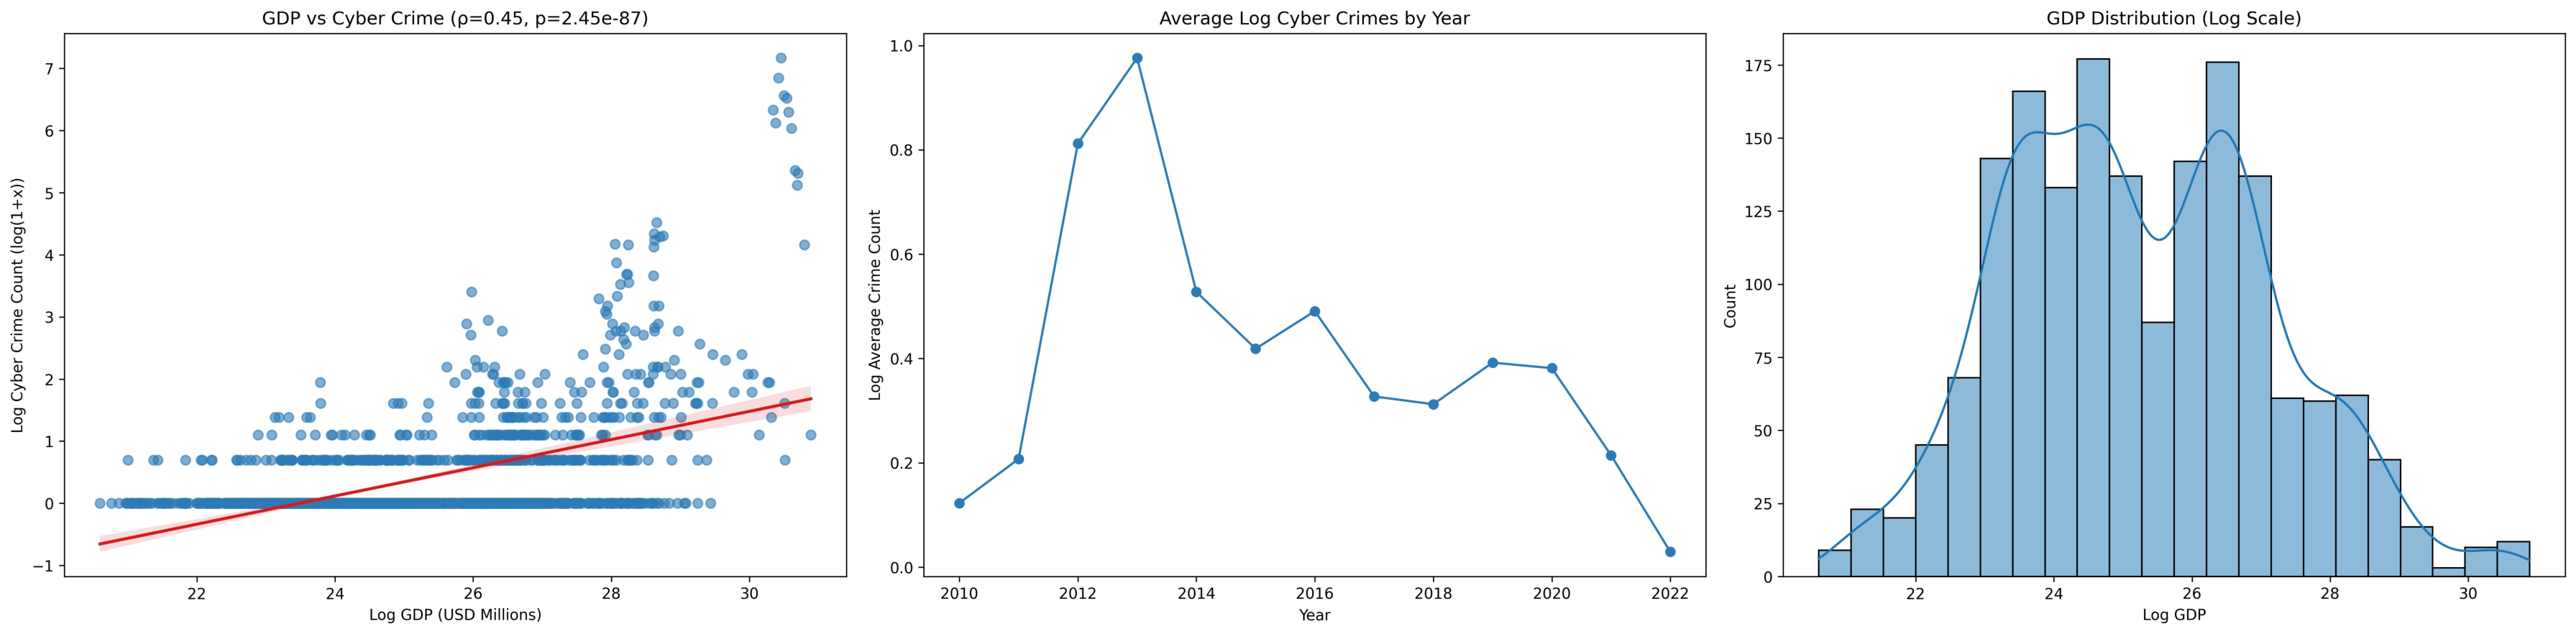
\includegraphics[width=1\linewidth]{../rsrc/demographics/gdp_crime_and_time}
            \caption{GDP Chart}\label{fig:gdp}
        \end{figure}

    \subsubsection{Distribution Plots} %5.3.3
        Finally, we generate distribution plots to examine the spread and density of the data.
        These plots illustrate the distribution of demographic indicators
        (e.g., internet user penetration, higher education enrollment) and their relationship with cybercrime counts.
        For example:
        \begin{itemize}
            \item The distribution plot for \textbf{internet user penetration} shows a right-skewed distribution,
                indicating that most countries have relatively low internet penetration rates.
                Figure~\ref{fig:internet}.
            \item The distribution plot for \textbf{higher education enrollment} reveals a more uniform distribution,
                with a peak around 60--80\% enrollment rates.
                Figure~\ref{fig:education}.
        \end{itemize}
        \begin{figure}[htbp]
            \centering
            \subfloat{
                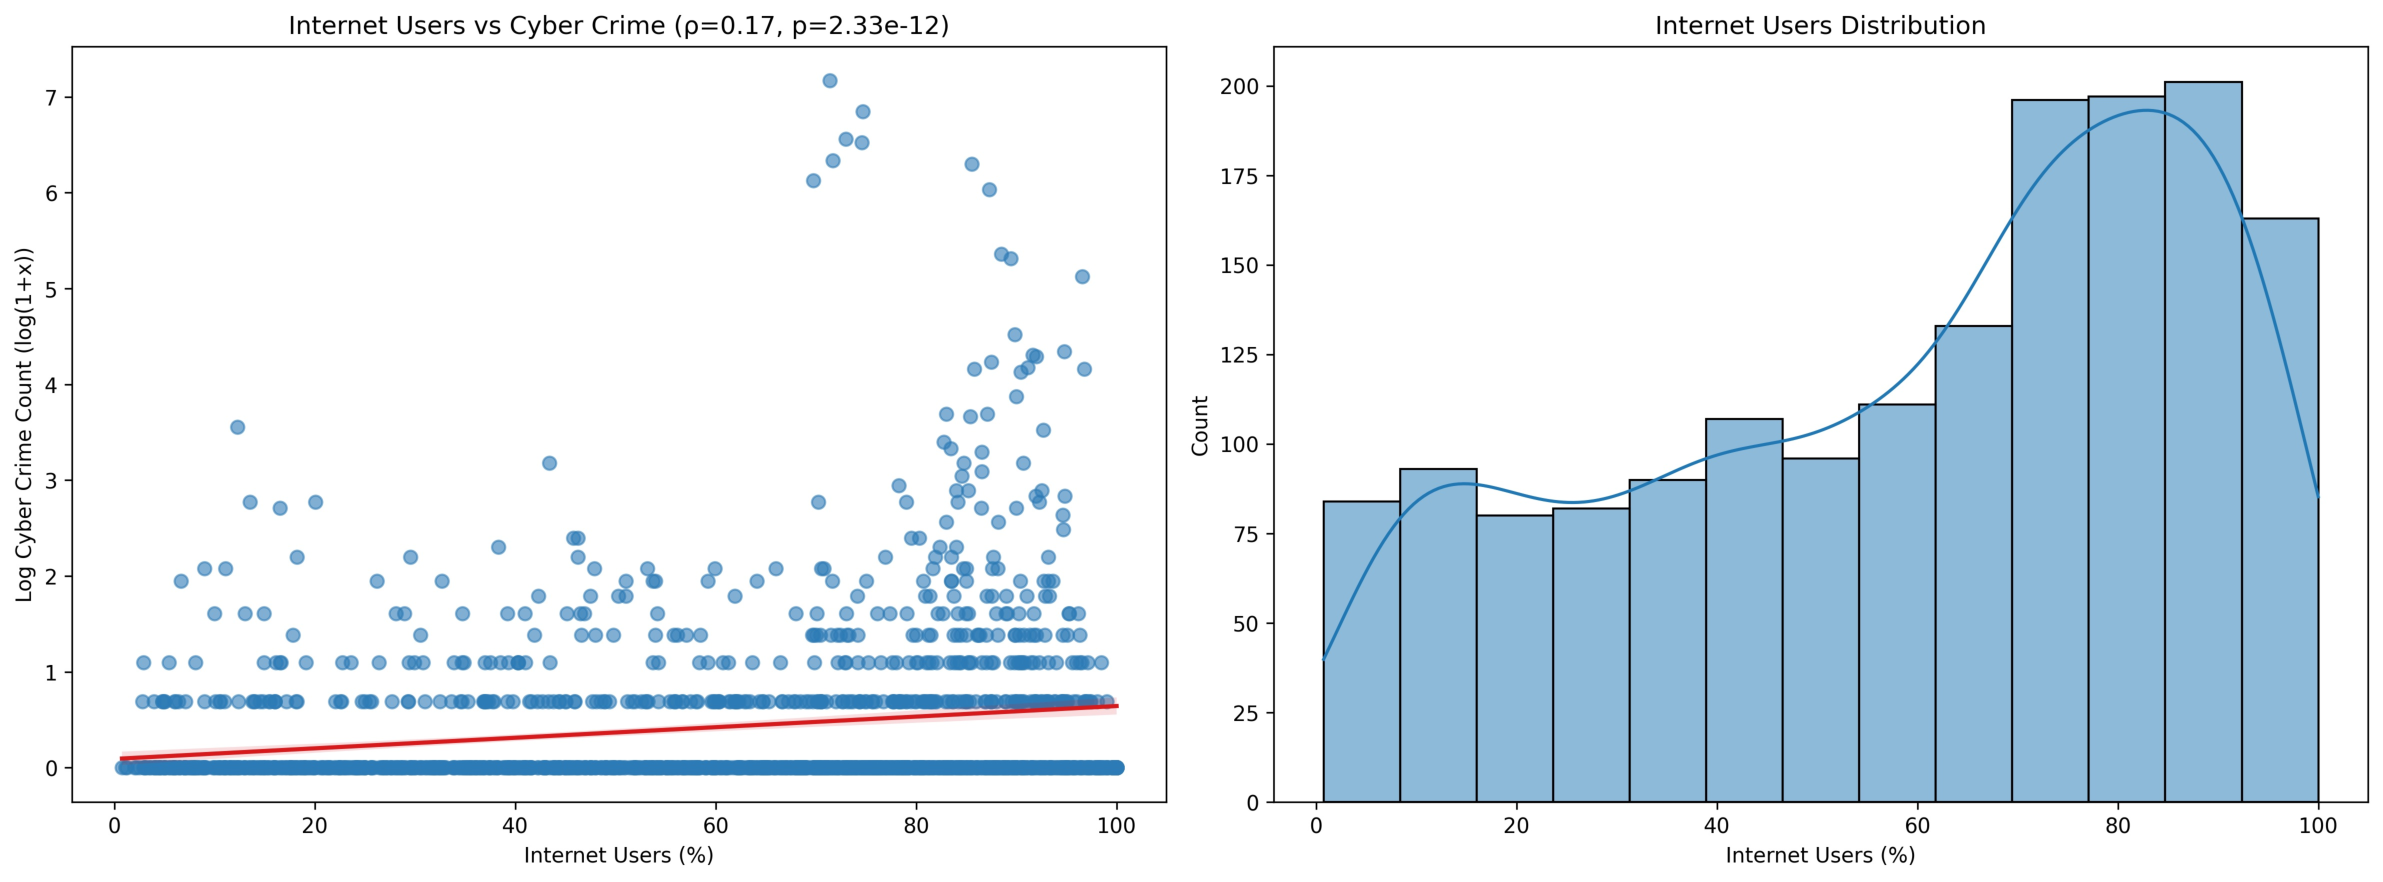
\includegraphics[width=0.8\linewidth]{../rsrc/demographics/Internet Users}\label{fig:internet}
            }\\
            \subfloat{
                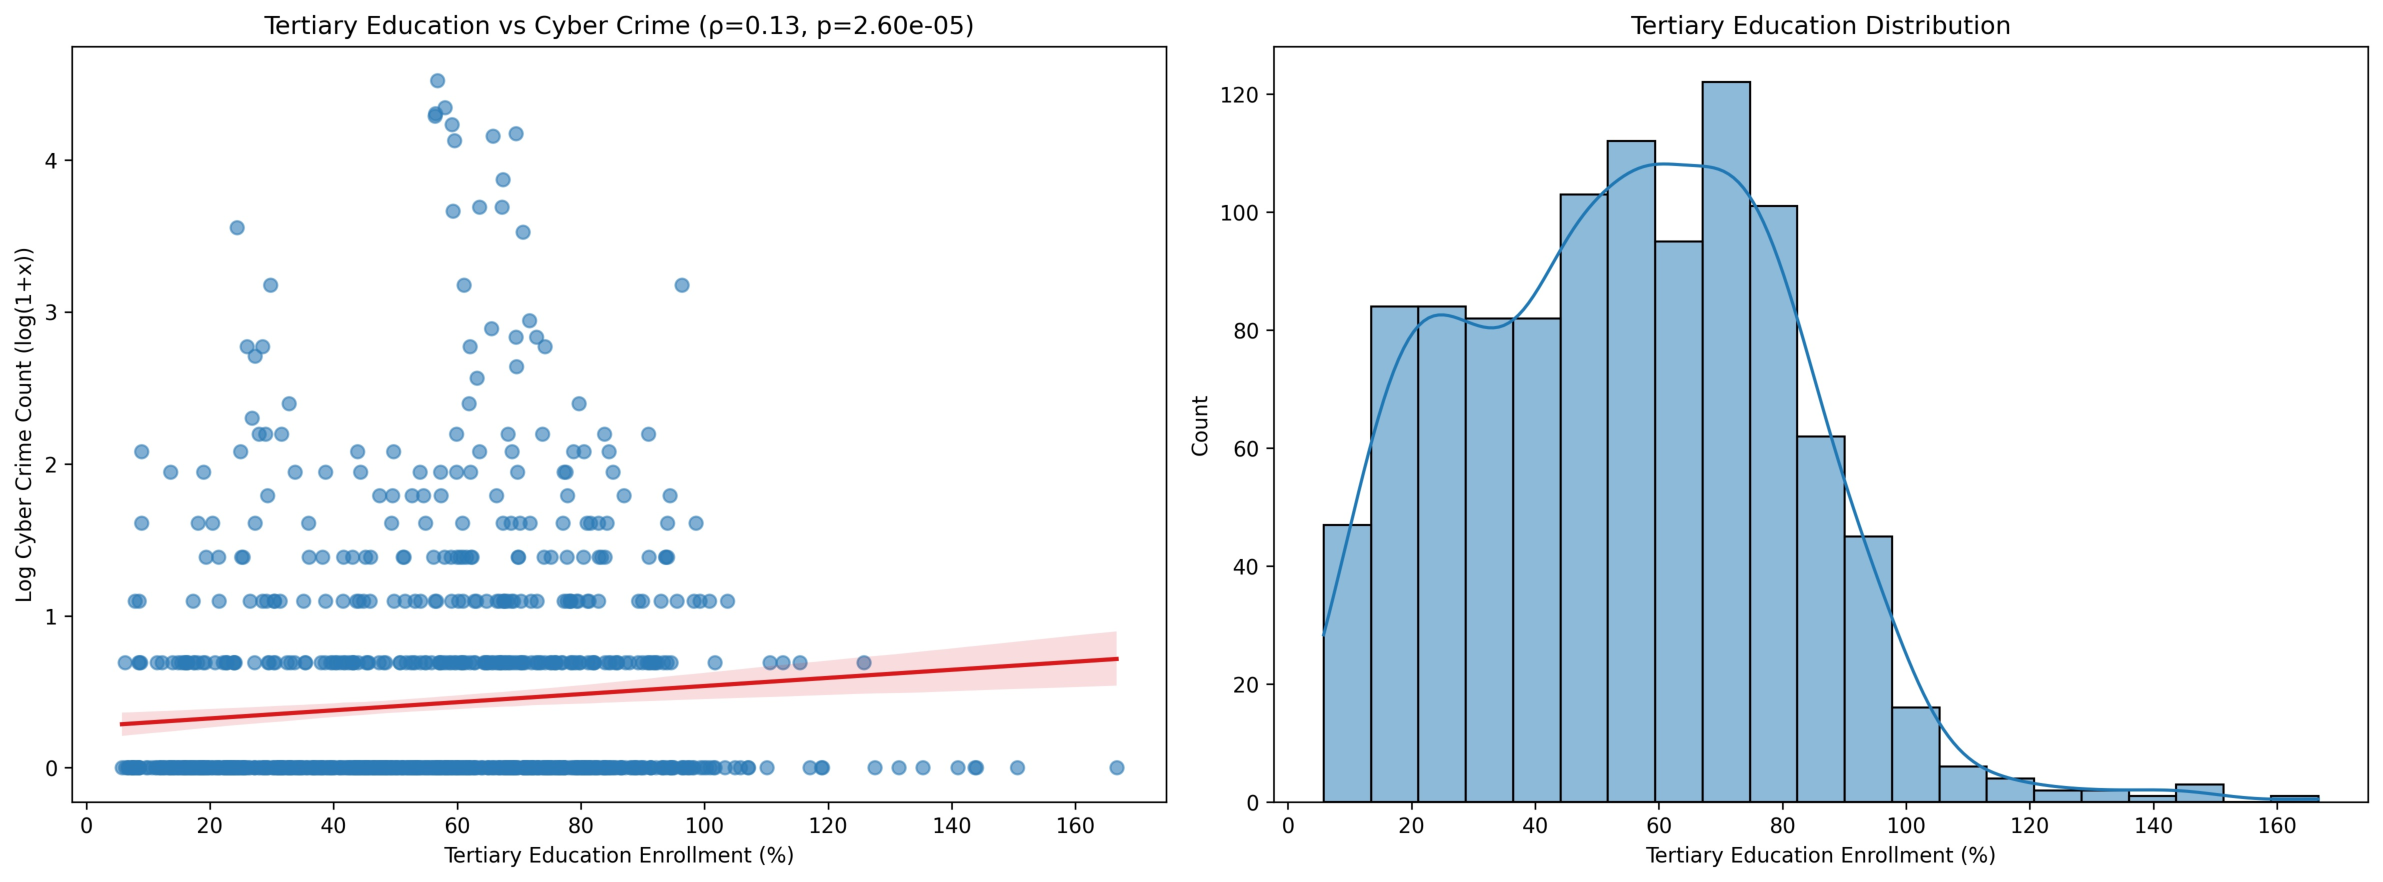
\includegraphics[width=0.8\linewidth]{../rsrc/demographics/Tertiary Education}\label{fig:education}
            }\\
            \caption{Trends and Correlations Related to Cybercrime}
        \end{figure}

    \subsubsection{Model Comparison: TOPSIS} %5.3.4
        \begin{enumerate}
            \item \textbf{Data Standardization}
                Standardize raw data to eliminate dimensional differences.
                For each indicator \(j\):
                - \textbf{Positive indicators} (higher values are better):
                \[
                    x_{ij}^* = \frac{x_{ij} - \min(x_j)}{\max(x_j) - \min(x_j)}
                \]
                - \textbf{Negative indicators} (lower values are better):
                \[
                    x_{ij}^* = \frac{\max(x_j) - x_{ij}}{\max(x_j) - \min(x_j)}
                \]
                where \(x_{ij}\) is the raw value of the \(i\)-th country for the \(j\)-th indicator.
            \item \textbf{Entropy-Based Weight Calculation} \\
                1. Calculate the probability distribution of standardized values:
                \[
                    p_{ij} = \frac{x_{ij}^*}{\sum_{i=1}^n x_{ij}^*}, \quad e_j = -\frac{1}{\ln n} \sum_{i=1}^n p_{ij} \ln p_{ij} \quad (p_{ij} \ln p_{ij} = 0 \text{ if } p_{ij}=0).
                \]
                2. Derive weights from entropy values:
                \[
                    w_j = \frac{1 - e_j}{\sum_{k=1}^m (1 - e_k)}.
                \]
            \item \textbf{Weighted Standardized Matrix}
                Construct the matrix \(V\) by combining standardized data with weights:
                \[
                    v_{ij} = w_j \cdot x_{ij}^*, \quad V = [v_{ij}]_{n \times m}.
                \]
            \item \textbf{Ideal Solutions}
                Define the ideal (\(S^+\)) and negative-ideal (\(S^-\)) solutions:
                \[
                    S^+ = \left\{ \max_{i}(v_{ij}) \mid j=1,2,\dots,m \right\}, \quad S^- = \left\{ \min_{i}(v_{ij}) \mid j=1,2,\dots,m \right\}.
                \]
            \item \textbf{Ranking via Relative Closeness} \\
                1. Calculate Euclidean distances to ideal solutions:
                \[
                    D_i^+ = \sqrt{\sum_{j=1}^m (v_{ij} - S_j^+)^2}, \quad D_i^- = \sqrt{\sum_{j=1}^m (v_{ij} - S_j^-)^2}.
                \]
                2. Compute relative closeness for ranking:
                \[
                    C_i = \frac{D_i^-}{D_i^+ + D_i^-}, \quad \text{where } C_i \in [0,1]. \quad (C_i \to 1 \text{ indicates better performance}).
                \]
        \end{enumerate}

        The Pearson correlation matrix (see Appendix~\ref{fig:correlation-matrix}) reveals critical insights into the relationships between key variables.
        Notably, \textbf{crime rates} exhibit a significant negative correlation with \textbf{education levels} (\(r = -0.13^*\)),
        suggesting that regions with higher educational attainment may experience reduced criminal activity, consistent with human capital theory.
        Similarly, \textbf{law enforcement intensity} (Warrant) shows a moderate negative association with crime rates (\(r = -0.25\)),
        reinforcing the deterrent effect of robust policing.
        The strongest observed correlation involves \textbf{risk prevention measures} (Risk),
        which display a pronounced negative relationship with crime rates (\(r = -0.50\) to \(-0.75\)),
        implying that targeted risk mitigation strategies could substantially curb criminal behavior.

        Among socioeconomic factors, \textbf{GDP} is positively correlated with \textbf{data reporting completeness} (\(r = 0.17^{**}\)),
        indicating that economically developed regions tend to have more reliable crime monitoring systems.
        Conversely, \textbf{internet penetration} demonstrates only a weak, non-significant link to crime rates (\(r = 0.1\)),
        highlighting its limited direct influence in the current model.

        \noindent \textit{Note: \(^*p < 0.05\), \(^{**}p < 0.01\). Variable definitions are provided in Appendix A.}

        \begin{figure}
            \centering
            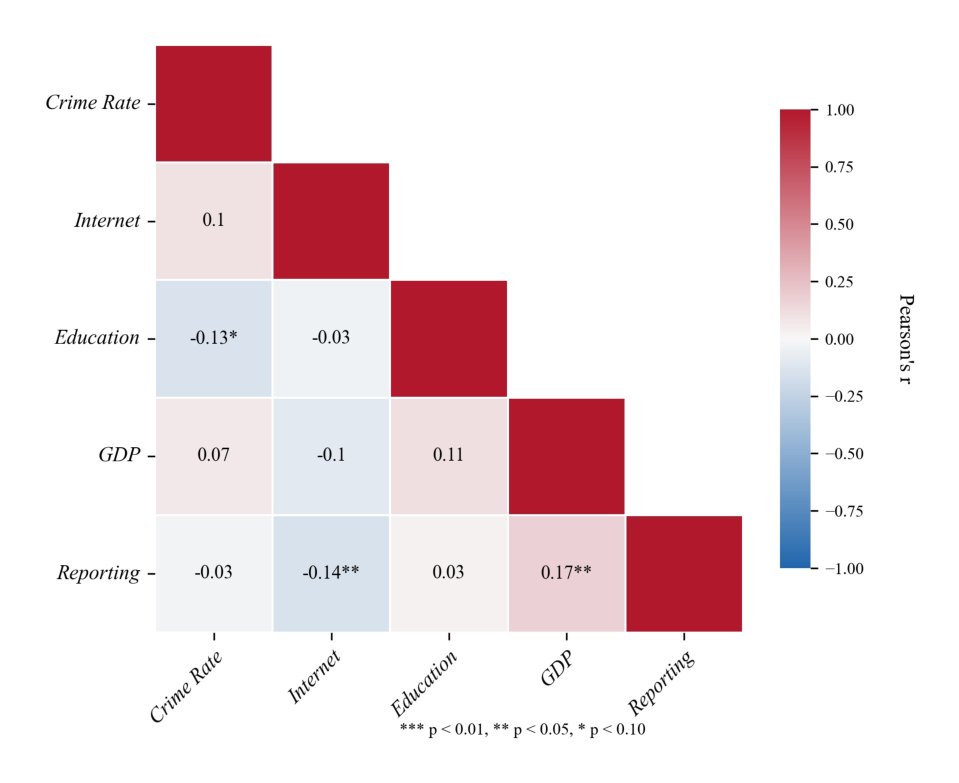
\includegraphics[width=0.75\linewidth]{../rsrc/demographics/correlation_matrix}
            \caption{Correlation Matrix}\label{fig:correlation-matrix}
        \end{figure}
